\documentclass[a4paper]{article}

\usepackage[T2A]{fontenc} % enable Cyrillic fonts
\usepackage[utf8]{inputenc} % make weird characters work
\usepackage{graphicx}

\usepackage[english,serbian]{babel}
\usepackage[unicode]{hyperref}

\usepackage{enumitem}
\usepackage{bm}
\usepackage{sfmath}
\usepackage{adjustbox}
\usepackage{multirow}

\begin{document}

New types of communication networks will be necessary to meet various consumer and regulatory
demands as well as satisfy requirements of safety and fuel efficiency. 
Multimedia systems will require high-bandwidth networks for
video transfer, and body electronics need low-bandwidth networks to keep the cost down.

\section{Protokoli komunikacije}
\label{sec:protokoli}

Računarske mreže u vozilima interno povezuje komponente unutar bilo koje vrste vozila. Svi uslovi koji bi trebalo da budu ispunjeni kada se govori o računarskim mrežama, poput sigurnosti u slanju poruka, rešavanje konflikta, minimalno vreme pristizanja poruka, efikasnost i slično, zahtevaju korišćenje protokola posebno definisanih za ovu problematiku. Različiti skupovi ovih modula zahtevaju različite tipove mreže. U današnjim vozilima postoje dva tipa mreže: veoma brze mreže za pogon i spore mreže za elektroniku u telu vozila. Podela mreže se vrši tako da predstavlja jednu lokalnu mrežu ili jednu funkcionalnu celinu. U ovim podeljenim mrežama, različiti delovi mreže mogu koristiti različite protokole. Na primer, jedna particija može da koristi CAN protokol, druga LIN protokol i tako dalje kao na slici \ref{fig:protokoliprimer}.

Osnovni zahtevi koji bi trebalo da budu ispunjeni su efikasno trošenje goriva, eliminisanje bregastih osovina u motoru i delova koji crpe energiju, nepotrebne težine vozila, povećanje sigurnosti. U vozilima se često koriste dve serijske magistrale, jedna za sistem koji kontroliše pogon, a druga za elektroniku u telu vozila. Proizvođači se trude da proizvedu što sigurnije vozilo i sa što boljim sistemom za upravljanje vozilom. U tabeli ~\ref{table:tabela1}  se može videti koje protokole koriste neki od proizvođača u zavisnosti od tipa vozila.

\begin{figure}[h]
\centering
 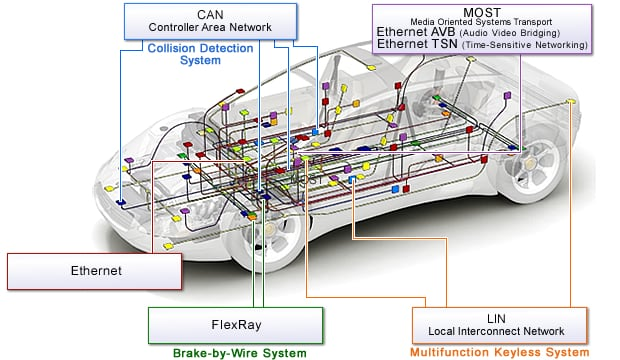
\includegraphics[width=0.9\textwidth]{protokoliprimer}
 \caption{Primer korišćenja protokola u automobilu}
 \label{fig:protokoliprimer}
\end{figure}


Postoje različiti tipovi protokola koji se mogu koristiti. Neki od tih protokola su:

\begin{itemize}

\item \textbf{CAN} - (Controller Area Network) Protokol koji se najčešće koristi kao LAN mreža vozila. Spada u sporu mrežu sa serijskom magistralom za prenos poruka, a koristi Non Return to Zero (NRZ) kodiranje. Sadrži 5 mehanizama za detekciju grešaka. % \cite{CAN}
\item \textbf{FlexRay} - Brza mreža koja omogućava visok stepen fleksibilnosti i pouzdanosti. Koristi point-to-point topologiju zvezde. Magistrala sa ovim protokolom dobro podnosi greške. % \cite{FlexRay}  
\item \textbf{LIN} - (Local Interconnect Network) Koristi se u serijskim magistralama koje se koriste za komunikaciju između inteligentnih senzora, ali i za elektroniku u telu automobila poput klima uređaja, vrata, sedišta i slično. % \cite{LIN}
\item \textbf{MOST} - (Media Oriented Systems Transport) Najčešći protokol kada su u pitanju multimedijalne mreže. Dizajniran tako da omogući prenos audio i video sadržaja kao i podataka visokog kvaliteta. % \cite{MOST}
\item \textbf{D2B} - (Domestic Digital Bus) Multimedijalni interfejs velike brzine. Koristi se u optičkim magistralama koje povezuju audio, video, kompijuterske i telefonske komponente u jednu prstenastu strukturu. % \cite{D2B}
\item \textbf{Byteflight} - Koristi se u sistemima koji se odnose na sigurnost (vazdušni jastuk). % \cite{Byteflight} 
\item \textbf{J1850} -Za deo vozila koji sadrži dijagnostičke aplikacije i aplikacije za deljenje podataka. % \cite{J1850} 
\item \textbf{IEBus} - Protokol zasnovan na CSMA/CD (Carrier Sense Multiple Access/Collision Detection) pristupu mreži. Prenos podataka se vrši kroz dve linije, Data+ i Data-, u dva smera. % \cite{IEBus} 
\item \textbf{J1708} - Koristi se samo u fizičkom sloju i to u serijskim magistralama, za komunikaciju između mikrokompjutera u vozilu. % \cite{J1708} 
\cite{viseujednom}

\item $\mathbf{A^{2}B}$ - (Automotive Audio Bus) Protokol audio distribucije. Ovim protokolom se dobija visoka vernost zvuka (Hi-Fi) uz smanjenje težine kablova i veće efikasnosti u trošenju goriva.  \cite{AB}
\item \textbf{AFDX} \cite{AFDX} 
\item \textbf{DC-BUS} \cite{DC-BUS} 
\item \textbf{IDB-1394} \cite{IDB-1394} 
\item $\mathbf{I^{2}C}$ \cite{IC}  
\item \textbf{ISO 9141-1/-2} \cite{ISO 9141-1/-2} 
\item \textbf{Keyword Protocol 2000} \cite{KeywordProtoco} 
\item \textbf{VAN} - (Vehicle Area Network) \cite{VAN}

\end{itemize}

Sledeće što se u budućnosti očekuje jeste povezivanje komponenti preko Web-a upravo zato što se količina podataka koje treba prenositi raste vremenom. Računarska mreža u vozilima konstantno se nadograđuje. Najverovatnije će se u vozila ubaciti sistemi zasnovani na Ethernet-u. Svaka komponenta vozila će imati svoju IP adresu tako da centralizovani računar i ruter u vozilu mogu da šalju i usmeravaju velike količine podataka. Ono što usporava ovakav razvitak jesu veliki troškovi, ali se takva nadogradnja očekuje jednog dana.

\begin{table}[h!]
\begin{center}
  
\begin{tabular}{ c|c|c|c }
\textbf{Tip protokola} & \textbf{Godina početka} & \textbf{Proizvođač} & \textbf{Tip vozila}\\
\hline
CAN & 1986 & Bosch & razno\\ \hline
\multirow{3}{*}{J1850} & \multirow{2}{*}{-} &  GM & \multirow{12}{*}{automobili} \\
	  & & Ford & \\ \cline{2-3}
             & \multirow{4}{*}{2008} & Chrysler &  \\ \cline{1-1} \cline{3-3}
\multirow{4}{*}{FlexRay}  &    & BMW &  \\
	 		 	 &    & Volkswagen &\\
				 &    & Daimler AG &\\   \cline{2-3}
				 &  - & General Motors &\\ \cline{1-3}
\multirow{4}{*}{MOST} & \multirow{4}{*}{?} & Ford  & \\ 
 &  & BMW & \\ 
 &  & Daimler& \\
 &  &  GM & \\ \cline{1-3}
 & 2000 & PSA Peugeot Citroën & \\ \hline
J1708 & 1985 & Volvo AB & teški terenac \\ \hline


\end{tabular}
\caption{Koje protokole koriste neki od proizvođača}
\label{table:tabela1}
\end{center}
\end{table}






\begin{thebibliography}{20}

\bibitem{viseujednom}
Automotive Buses
\url{http://www.interfacebus.com/Design_Connector_Automotive.html}
11.5.2018.

\bibitem{AB} 
Analog Devices.
\textit{A better design experience. A more dynamic automotive experience. ADI's $\mathbf{A^{2}B}$ technology delivers both.}
\url{http://www.analog.com/en/landing-pages/001/a2b.html}. 
Analog Devices, 11.5.2018.
 
\bibitem{AFDX}
\textit{Avionics Full-Duplex Switched Ethernet.}
\url{https://en.wikipedia.org/wiki/Avionics_Full-Duplex_Switched_Ethernet}. 
11.5.2018.
 
\bibitem{DC-BUS} 
\textit{DC BUS Technology.}
\url{http://yamar.com/power-line-communication/}.
11.5.2018.

\bibitem{IDB-1394} 
\textit{IDB-1394.}
\url{https://en.wikipedia.org/wiki/IEEE_1394#IDB-1394}.
11.5.2018.

\bibitem{IC}
\textit{Inter-Integrated Circuit.}
\url{https://en.wikipedia.org/wiki/I\%C2\%B2C}.
11.5.2018.

\bibitem{ISO 9141-1/-2}
\textit{ISO 9141.}
\url{https://en.wikipedia.org/wiki/On-board_diagnostics#ISO_standards}.
11.5.2018.

\bibitem{KeywordProtoco}
\textit{Keyword Protocol 2000.}
\url{https://en.wikipedia.org/wiki/Keyword_Protocol_2000}.
11.5.2018.

\bibitem{VAN}
\textit{Vehicle Area Network.}
\url{https://en.wikipedia.org/wiki/Vehicle_Area_Network}.
11.5.2018.

\bibitem{LIN}
\textit{Local Interconnect Network.}
\url{https://en.wikipedia.org/wiki/Local_Interconnect_Network}.
11.5.2018.

\bibitem{MOST}
\textit{IDB-1394.}
\url{https://en.wikipedia.org/wiki/IEEE_1394#IDB-1394}.
11.5.2018.

\bibitem{Byteflight} 
\textit{Byteflight.}
\url{https://en.wikipedia.org/wiki/Byteflight}.
11.5.2018.
 
\bibitem{CAN} 
\textit{Controller Area Network.}
\url{https://en.wikipedia.org/wiki/CAN_bus}.
11.5.2018.

\bibitem{D2B} 
\textit{Domestic Digital Bus.}
\url{https://en.wikipedia.org/wiki/Domestic_Digital_Bus_(automotive)}.
11.5.2018.

\bibitem{FlexRay} 
\textit{FlexRay.}
\url{https://en.wikipedia.org/wiki/FlexRay}.
11.5.2018.

\bibitem{IEBus}
\textit{Inter Equipment Bus.}
\url{https://en.wikipedia.org/wiki/IEBus}.
11.5.2018.
\bibitem{J1708}
\textit{SAE J1708.}
\url{https://en.wikipedia.org/wiki/SAE_J1708}.
11.5.2018.

\bibitem{J1850}
\textit{SAE J1850.}
\url{https://en.wikipedia.org/wiki/On-board_diagnostics#SAE_standards_documents_on_OBD-II}.
11.5.2018.



\end{thebibliography}




\end{document}
